
\chapter{Continuous transfer in Deep Q-learning}
\label{sec:continuous}

In this chapter, we include a \idx{transfer} process inside the workflow of a \acrfull{DQN} algorithm. As stated in \Cref{chapter:dm-tl}, a \acrfull{TL} algorithm consists of two phases, a \textit{\idx{transfer}} phase where we choose what or how to \idx{transfer}, and a \textit{learning} phase where we learn the target policy using the \idx{transfer}red knowledge. There are different ways of implementing those phases in the \gls{DQN} algorithm; we introduce some of them that failed in practice, and we explain why. First, we describe briefly how \gls{DQN} works.


\subsection{Deep Q-learning} \gls{DQN} is an \idx{Online} \acrfull{RL} algorithm fit for continuous state-space and discrete action-space. It uses a \acrfull{NN} as $\Q$-function approximator. One can see \gls{DQN} as an adaptation of the $\Q$-learning algorithm using a \gls{NN} as function approximator. Indeed, \gls{DQN} updates the weights online with respect to the \acrfull{TD} error. In order to remember its previous interactions with the \idx{environment}, \gls{DQN} keeps the \idx{transition}s in a memory called the Experience Replay. So, instead of considering a single interaction to update the weights, \gls{DQN} draws a random set of previously encountered interactions\footnote{In order to makes the data fed to the neural network \gls{iid}.}, called the replay buffer, and computes the mean \gls{TD} error over those interactions. To ensure stability, \gls{DQN} is equipped with two networks:

\begin{itemize}
    \item the \textit{\idx{greedy}} network, updated at each interaction, is used to compute the \idx{greedy} action in order to interact with the \idx{environment}.
    \item the \textit{bootstrap} network\footnote{In the literature, this network is called \textit{target} network, but this nomenclature conflicts with the idea of target \idx{environment} and target policy bought by the \gls{TL} framework.}, updated at a lower frequencies, is used to compute the argument of $\max$ operator in the \gls{TD} error.
\end{itemize}

Now we identified the different components of \gls{DQN}, we are able to incorporate \idx{transfer} knowledge into it. Now let us assume that we are given a set of different \idx{user}s $\users$. For any $u\in\users$, we know the optimal \gls{DP} (and underlying \idx{greedy} network) $\policy_u$ and the \idx{batch} of interactions $\cD_u$ used to learn the \gls{DP}.

\section{The transfer phase.}

First, to operate the \textit{\idx{transfer}} phase, we investigate two ideas to choose what source we \idx{transfer} from:

\subsection{Auto-Encoders}

 For each \idx{user} $u$, we learn an Auto-Encoder $AE_u$ that reconstruct the \idx{transition}s contained in $\cD_u$. The learning \idx{batch} takes this form:
 $\{t_{\indextransition},t_{\indextransition}\}_{{\indextransition}\in[0,|\cD_u|[}$
 %!TU: Ok mais ca me surprend. Pour modeliser l'utilisateur $u$ j'aurai plutot envie d'apprendre $P_u$ sur des paires $[(s_i,a_i) -> (r_i,s'_i)]$$
%NC: ne fonctionne pas si l'environement est stochastique
 where $t$ is a concatenation of corresponding interaction's components: $t_{\indextransition}= (s_{\indextransition},a_{\indextransition},r_{\indextransition}',s_{\indextransition}')$. Then to select the closest source \idx{user} to the target \idx{user}, we forward the target interactions in each source Auto-Encoder and compute the test error. We postulated at first that the lowest test error would correspond to the closest source \idx{user}. That statement showed promising results on a cart-pole \idx{environment} and on PyDial. Unfortunately, the discriminative attribute that helped to select the best source was mostly the action. That makes sense when we think that the learning of the Auto-Encoder is actually biased by the action distribution in the \idx{batch}, that is conditioned by the policy that generated this \idx{batch}. Another limit of this approach is the fact that the Auto-Encoder may not really capture the transition function $\transition$ as it may learn to reconstruct each $s$  and $s'$ independently if occurrences of any of those are high enough. One solution might be using the algorithm proposed in \textcite{ammar2014automated} based on \glspl{RBM}, but they only encode $(s_{\indextransition},a_{\indextransition},s_{\indextransition}')$.

\subsection{Using the Temporal Difference error}

Here, we consider each source \idx{greedy} $\Q$-network. To select the closest source \idx{user}, we compute the \gls{TD} error of each source \idx{greedy} network using the target \idx{batch} of \idx{transition}s. We made the hypothesis that the network that minimises this error may perform better with the target environment. This statement is false and we propose a simple counter example where the network with the lowest \gls{TD} error is sub-optimal. Consider the simple target \gls{MDP} in \Cref{fig:counter-exemple-td} where the starting state is $s$. As the \gls{MDP} is \idx{deterministic} and there are only two actions, we can represent a transition using its reward. So we assume the target \idx{batch} $\cD_{u_t} = \{1,0\}$. Now let us say we have two source networks, $\Q_{u_0}$ and $\Q_{u_1}$, and let $\Q_{u_0}(a_0) = -1$, $\Q_{u_0}(a_1) = 0$, $\Q_{u_1}(a_0) = 5$ and $\Q_{u_1}(a_1) = 0$. Then the average \gls{TD} error of $\Q_{u_0}$ w.r.t $\cD_{u_t}$ is $1$ and the average \gls{TD} error of $\Q_{u_1}$ is $2$. So $\Q_{u_0}$ seems better than $\Q_{u_1}$, however, the policy based on $\Q_{u_0}$ will always choose $a_1$ the sub-optimal action $a_1$ while the policy based on $Q_{u_1}$ will always choose the best action $a_0$.

\begin{figure}
    \begin{center}
        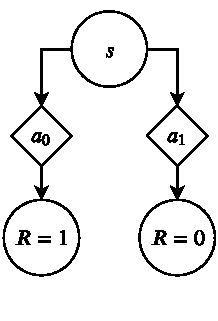
\includegraphics[width=0.25\textwidth,page=1]{sources/conclusion/mdp}
    \end{center}
    \caption[Counter example for the Temporal Difference error solution]{Counter example Markov Decision Process of the Temporal Difference error solution}
    \label{fig:counter-exemple-td}
\end{figure}

\section{The learning phase}

We also proposed two solutions for learning the policy through \gls{DQN} using the \idx{transfer}red knowledge. Two questions arise, what data to \idx{transfer} and when to stop the \idx{transfer}.

\subsection{Transferring the transition}

In this solution, we tried to \idx{transfer} the \idx{transition}s of the best current source \idx{user} (using the source selection of our choice, at this moment, we used the Auto-Encoder method). To operate the \idx{transfer}, we simply fill up the remaining space of the replay buffer with the source \idx{transition}s. That way, the target \gls{DQN} includes source knowledge into its learning. The advantage of this method is that once the replay buffer is full of target \idx{transition}s, there is no more need to \idx{transfer} source knowledge. Thus, there is no need to control the \idx{transfer} through a meta parameter. The direct drawback of this, since replay buffer rarely exceeds 128 \idx{transition}s, is that the target \gls{DQN} prematurely stops using the source knowledge and the benefit of the \idx{transfer} is not exploited enough. Another lead of research could be adding the \idx{transition}s into the target experience replay directly, and clean it from source \idx{transition}s at some point of the learning to avoid negative \idx{transfer}. In this case, the question would be when to stop the \idx{transfer}. Finally, all methods \idx{transfer}ing the \idx{transition}s face a major issue: at the very beginning of the learning, the policy is sub-optimal as it dit not have the time to bootstrap. \textcite{laroche2019} showed recently that vanilla \gls{DQN} is actually bad at batch learning. That led us to the next solution, that is \idx{transfer}ing directly the $\Q$-network.


\subsection{Transferring the network}

We tried two solutions for \idx{transfer}ring the network.

The first one relies on a simple idea: using the network that minimise the \gls{TD} error among all the source networks and the target network. As the target \idx{greedy} network is learnt on the \idx{batch} he is tested on, we must learnt an extra target network on a partial part of the \idx{batch}, the learning base, and test it on the other part, the test base. The idea is similar to slice the learning \idx{batch} in \acrfull{SL} problems. Unfortunatly, as we saw with the counterexample in \Cref{fig:counter-exemple-td}, the \gls{TD} is not an appropriate metric to evaluate what network is the best fit for the target environment.

The second solution consists on concatenating the current best source network (using the source selection of our choice) and the target network and weight their output in a single meta-network. The basic idea is to freeze the gradient of the source network and only learn the weights of the gate (that weights the output of the source and target network) and the weights of the \idx{greedy} target. We also add extra information for the gate, as for example, the error return by the source Auto-Encoder. We believe that the meta-network should be able to emphasise the source network when the learning \idx{batch} of the target \idx{environment} is small and emphasise the target network when it is strong enough to minimise the \gls{TD} error. But once again, the foundation of the idea also relies on the fact that a small \gls{TD} error should indicate a good fit for the target environment which is false.

\section{Conclusion}

The idea of \idx{transfer}ring knowledge continuously into \gls{DQN} is very tempting, convenient and does not need many changes to fit the initial framework. However, the \idx{Online} nature of the algorithm makes it very hard to select the right source knowledge to \idx{transfer} as the processus is not stationary. The two main challenges rely on what source to pick, and when to stop the \idx{transfer}. We consider at the moment learning the $\reward$ and $\transition$ function using ideas from the \idx{model-based} community~\parencite{Deisenroth2011} in order to detect the closest source environment. The idea of combining \idx{model} of the environments and a \idx{model-free} algorithm may be counter-intuitive and unproductive, so a switch to a \idx{model-based} algorithms may be appropriate.

\subsection{Discussion}

A lot of related work has been conducted since the beginning of this work. The closest of ours is \textcite{chaplot2016transfer} where the authors transfer the features of the \gls{DQN} model on DOOM 3d environment. To cite a few another recent works: Model-Agnostic Meta-Learning~\parencite{finn2017model} for \gls{RL} on MuJoCo; Successor Features - a generalisation of Successor Representations~\parencite{dayan1993improving} -  on the DeepMind Lab platform~\parencite{barreto2019transfer}, or on robot navigation tasks~\parencite{zhang2017deep}; generalisation through simulation~\parencite{kang2019generalization} for vision-based autonomous flight.

%!TU: Ca ira tout a fait pour la soutenance de these, mais la partie sur le TL
% me parait franchement incomplete
% Il manque un vrai travail de formalisation du probleme. On pourra en reparler si tu veux mais je suis convaincu que ce genre de probleme se modeliserait plus naturellement avec des POMDP et des "belief-states".
